\documentclass[a4paper,norsk,11pt]{interaktiv}
\usepackage{tcolorbox}
% Importerte pakker
\usepackage{float}
\restylefloat{figure}
\usepackage{ifluatex}
\usepackage{subfigure}
\usepackage{tikz}
\usetikzlibrary{arrows}
\usepackage[parfill]{parskip}    		% Activate to begin paragraphs with an empty line rather than an indent
\usepackage{graphicx}
\usepackage[standard-baselineskips]{cmbright}

\newcommand{\V}[1]{\mathbf{#1}}
\usepackage{unicode-math}

\ifluatex
  \usepackage{fontspec}
  \setmainfont{Calibri}
  \usepackage{unicode-math}
  \setmathfont{Cambria Math}
\else
  \usepackage[utf8]{inputenc}
\fi

\usepackage[european,americanvoltages]{circuitikz}

\usepackage{url}

\newenvironment{amatrix}[1]{% "augmented matrix"
  \left[\begin{array}{*{#1}{c}|c}
}{%
  \end{array}\right]
}
% Underfigurer
\renewcommand{\thesubfigure}{(\arabic{subfigure})}

% Overskrift
\emnekode{TMA4101}
\emnenavn{Matematikk 1 for MTELSYS}




% Nye kommandoer
\newcommand{\dee}{\mathop{}\!{d}}


\title{Lineære likningssystemer I}



\begin{document}
\pagenumbering{gobble}

\maketitle

Velkommen til øvingsopplegget i TMA4101. 

Opplegget er organisert i samme ånd som i TTT4203 - hver øving skal gi deg erfaring og trening, 
samt stimulere til refleksjon. 
Øvingene er ikke obligatoriske, 
men matematikk er et modningsfag, 
og skippertak før eksamen vil ikke være tilstrekkelig for en god karakter.



\section*{Standardoppgaver}


%\begin{oppgave}{E1}
%Lag et pythonscript som plotter eksponensialfunksjonen på intervallet $[-1,1]$.
%\end{oppgave}


\begin{oppgave}{S1}
Løs likningssystemet
\[
\setlength\arraycolsep{1pt}
\begin{array}{rcrcrcrc@{\qquad}l}
3x_1  &  - &   x_2    & - &   x_3   &  &      &   =   &  1  \\
-x_1 & + &   3x_2   &  &     & - &   x_4   &   =   &  0 \\
-x_1 &    &        & +  &   3x_3  &  - &   x_4   &  =   &   0\\
   &  - &   x_2   &  - &    x_3   &  + &   3x_4   &  =   &  0 
\end{array}
\]
som best du kan.
\end{oppgave}

Hvis du lærte det samme som jeg (født i 1983) på ungdomsskolen,
brukte du antagelig innsettingsmetoden i oppgaven over.
Det finnes tusenvis av forskjellige teknikker for å løse veldig spesialiserte lineære likningssystemer, 
men metoden alle universitetskurs begynner med, 
kalles gausseliminasjon.

\url{https://en.wikipedia.org/wiki/Gaussian_elimination}



\begin{oppgave}{S2}
Løs likningssystemet
\[
\setlength\arraycolsep{1pt}
\begin{array}{rcrcrcrc@{\qquad}l}
3x_1  &  - &   x_2    & - &   x_3   &  &      &   =   &  1  \\
-x_1 & + &   3x_2   &  &     & - &   x_4   &   =   &  0 \\
-x_1 &    &        & + &   3x_3  &  - &   x_4   &  =   &   0\\
   &  - &   x_2   &  - &    x_3   &  + &   3x_4   &  =   &  0 
\end{array}
\]
med gausseliminasjon.
\end{oppgave}

Gausseliminasjon ble oppfunnet av noen kinesere for omtrent to tusen år siden. 
Men gausseliminasjon er bare starten på alt;
lineære likningssystemene er springbrett for et kjempestort matematisk fagfelt som kalles algebra:

\url{https://en.wikipedia.org/wiki/Algebra}

Vi trenger ikke studere abstrakt algebra helt ennå.
Men de første par ukene i semesteret, 
skal vi studere teorien bak lineære likningssystemer:

\url{https://en.wikipedia.org/wiki/System_of_linear_equations}



Et lineært system i en moderne anvendelse kan fint ha en en million likninger og ukjente. 
Det sier seg selv at dette ikke kan løses for hånd.

\begin{oppgave}{S3}
Løs likningssystemet
\[
\setlength\arraycolsep{1pt}
\begin{array}{rcrcrcrc@{\qquad}l}
3x_1  &  - &   x_2    & - &   x_3   &  &      &   =   &  1 \\
-x_1 & + &   3x_2   &  &     & - &   x_4   &   =   &  0 \\
-x_1 &    &        & + &   3x_3  &  - &   x_4   &  =   &   0\\
   &  - &   x_2   &  - &    x_3   &  + &   3x_4   &  =   &  0 
\end{array}
\]
i python.
\end{oppgave}



\section*{Viderekomne oppgaver}

Her kommer først en veldig enkel en. 
Det skal i neste uke bli klart hvorfor den er så enkel.

\begin{oppgave}{V1}
Løs likningssystemet
\[
\setlength\arraycolsep{1pt}
\begin{array}{rcrcrcrc@{\qquad}l}
3x_1  &  - &   x_2    & - &   x_3   &  &      &   =   &  0  \\
-x_1 & + &   3x_2   &  &     & - &   x_4   &   =   &  0 \\
-x_1 &    &        & +  &   3x_3  &  - &   x_4   &  =   &   0\\
   &  - &   x_2   &  - &    x_3   &  + &   3x_4   &  =   &  0 
\end{array}
\]
\end{oppgave}

De neste tre systemene er av en type du mest sannsynlig ikke har sett før.

\begin{oppgave}{V2}
Løs likningssystemet
\[
\setlength\arraycolsep{1pt}
\begin{array}{rcrcrcrc@{\qquad}l}
3x_1  &  - &   x_2    & - &   x_3   &  &      &   =   &  0  \\
-x_1 & + &   3x_2   &  &     & - &   x_4   &   =   &  0 \\
-x_1 &    &        & + &   3x_3  &  - &   x_4   &  =   &   0\\
 x_1  &  + &   2x_2   &  + &    2x_3   &  + &   x_4   &  =   &  0 
\end{array}
\]
\end{oppgave}

\begin{oppgave}{V3}
Løs likningssystemet
\[
\setlength\arraycolsep{1pt}
\begin{array}{rcrcrcrc@{\qquad}l}
3x_1  &  - &   x_2    & - &   x_3   &  &      &   =   &  1  \\
-x_1 & + &   3x_2   &  &     & - &   x_4   &   =   &  1 \\
-x_1 &    &        & + &   3x_3  &  - &   x_4   &  =   &   1\\
 x_1  &  + &   2x_2   &  + &    2x_3   &  + &   x_4   &  =   &  3 
\end{array}
\]
\end{oppgave}

\begin{oppgave}{V4}
Løs likningssystemet
\[
\setlength\arraycolsep{1pt}
\begin{array}{rcrcrcrc@{\qquad}l}
3x_1  &  - &   x_2    & - &   x_3   &  &      &   =   &  1  \\
-x_1 & + &   3x_2   &  &     & - &   x_4   &   =   &  1 \\
-x_1 &    &        & + &   3x_3  &  - &   x_4   &  =   &   1\\
 x_1  &  + &   2x_2   &  + &    2x_3   &  + &   x_4   &  =   &  1 
\end{array}
\]
\end{oppgave}

\section*{Dagens fun fact}
Nord på kartet peker mot den geografiske nordpolen. 
Denne flytter seg ikke over tid, 
men den magnetiske nordpolen gjør. 
Forskjellen i grader mellom geografisk og magnetisk nordpol kalles misvisning,
og denne er viktig for båtførere.

Din kurs $\alpha$ relativt til geografisk nordpol kalles rettvisende kurs, 
og din kurs $\theta$ relativt til magnetisk nordpol, 
kalles magnetisk kurs. 
Misvisningen $m$ er sånn nogenlunde konstant innenfor et og samme sjøkart 
(den endrer seg betydelig langs norskekysten og med en grad eller to per tiår),
og disse tre tilfredsstiller den lineære likningen
\[
\alpha=\theta+m.
\]
Ved fravær av magnetisk påvirkning fra båten vil et magnetisk kompass peke mot den magnetiske nordpolen.
Dersom kompasset blir påvirket av interne magnetiske felt i båten,
får vi i tillegg noe som kalles deviasjon,
og alt blir litt mer komplisert.
Dette skal vi se på senere.

På sjøkart er likningen $x=y+a$ er fremstilt grafisk i kompassrosen, 
se figur. 
(Kartet under er fra Helgelandskysten.
Misvisningen var på 3 grader øst i 2015, 
og øker med omtrent en grad hvert sjette år.)
\begin{figure}
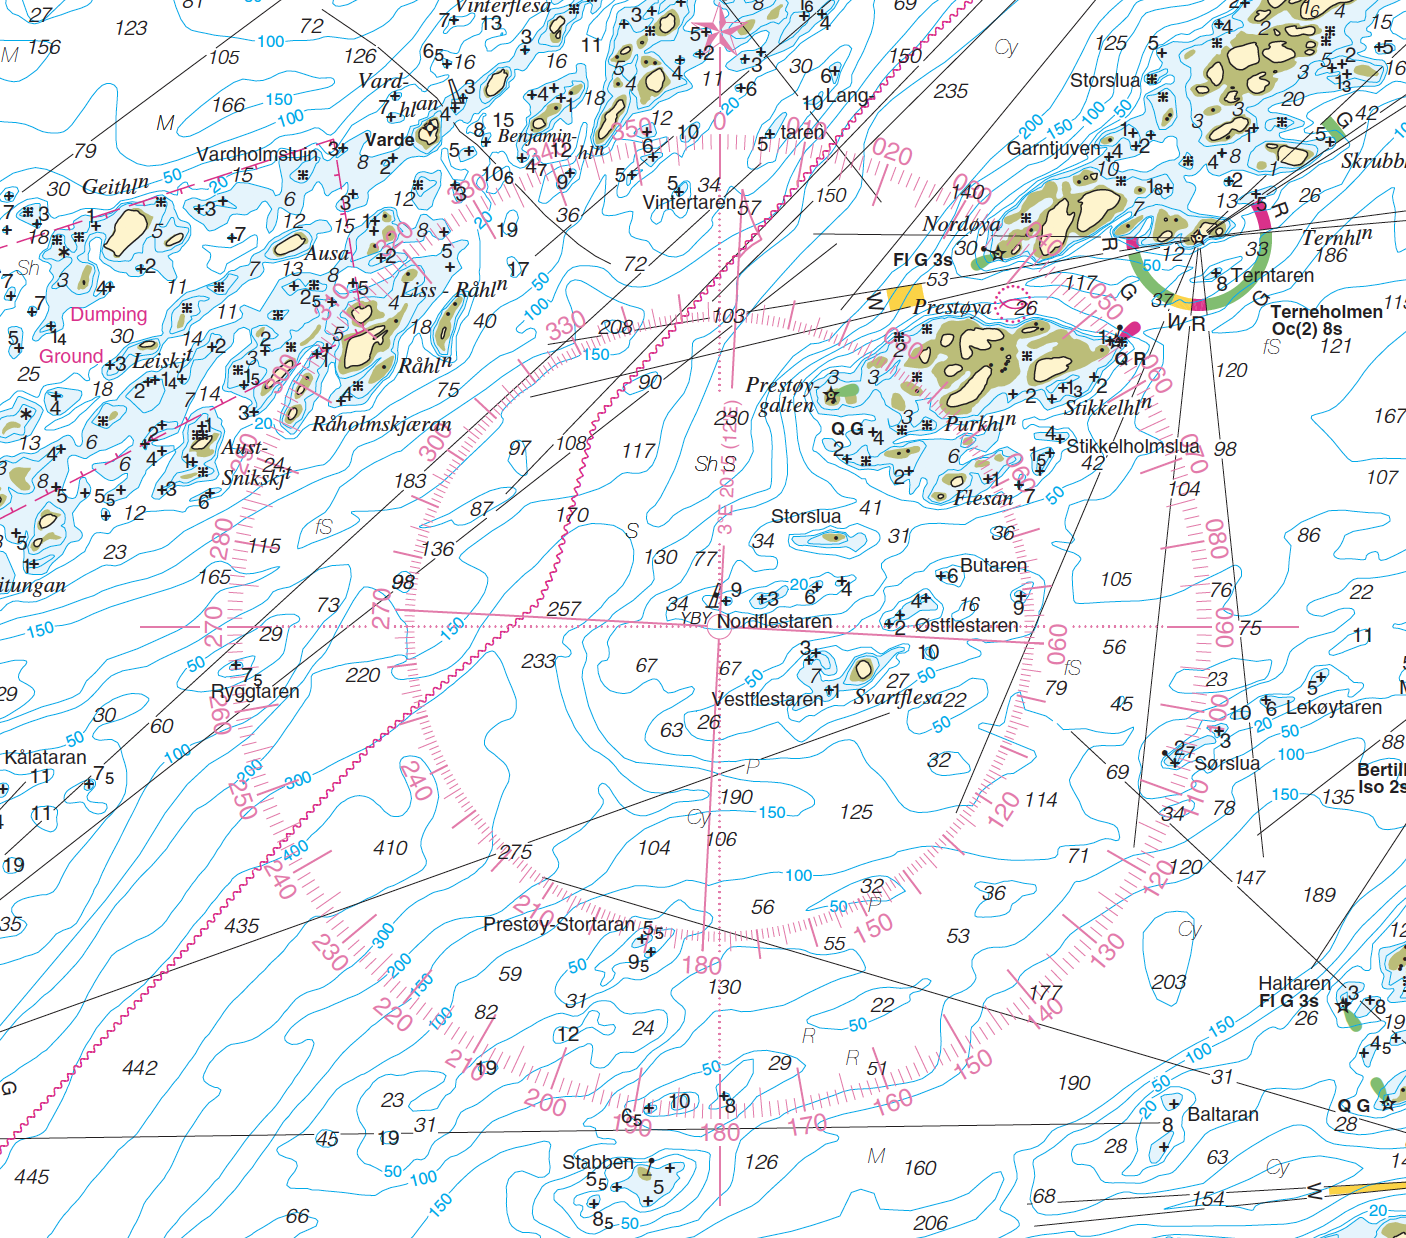
\includegraphics[scale=.67]{kompassrose}
\end{figure}


\end{document}
